\section{Thread Class Reference}
\label{class_thread}\index{Thread@{Thread}}
Inheritance diagram for Thread::\begin{figure}[H]
\begin{center}
\leavevmode
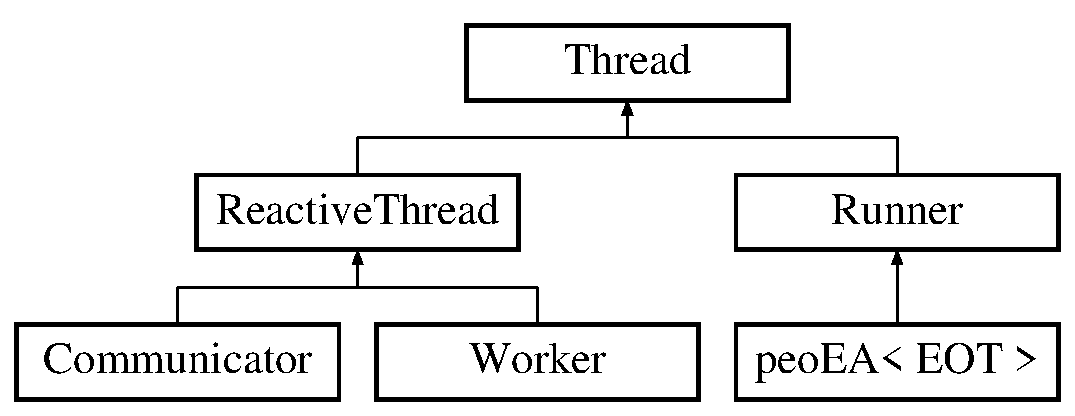
\includegraphics[height=3cm]{class_thread}
\end{center}
\end{figure}
\subsection*{Public Member Functions}
\begin{CompactItemize}
\item 
{\bf Thread} ()\label{class_thread_95c703fb8f2f27cb64f475a8c940864a}

\item 
virtual {\bf $\sim$Thread} ()\label{class_thread_37d9edd3a1a776cbc27dedff949c9726}

\item 
virtual void {\bf start} ()=0\label{class_thread_c667c1d8fd7243d669043e3dd762b567}

\item 
void {\bf set\-Active} ()\label{class_thread_e197c46f8f62ecce6d2a7fe95bdc5b38}

\item 
void {\bf set\-Passive} ()\label{class_thread_20632ffe9ddfa2a478afb0c84dc1096b}

\end{CompactItemize}
\subsection*{Private Attributes}
\begin{CompactItemize}
\item 
bool {\bf act}\label{class_thread_1b155d63bca3096ac4a1d039aea83c7c}

\end{CompactItemize}


\subsection{Detailed Description}




Definition at line 31 of file thread.h.

The documentation for this class was generated from the following files:\begin{CompactItemize}
\item 
thread.h\item 
thread.cpp\end{CompactItemize}
